\begin{scanpage}{0135}{117}
\noindent\begin{minipage}[t]{.48\linewidth}\vspace{0pt}\centering
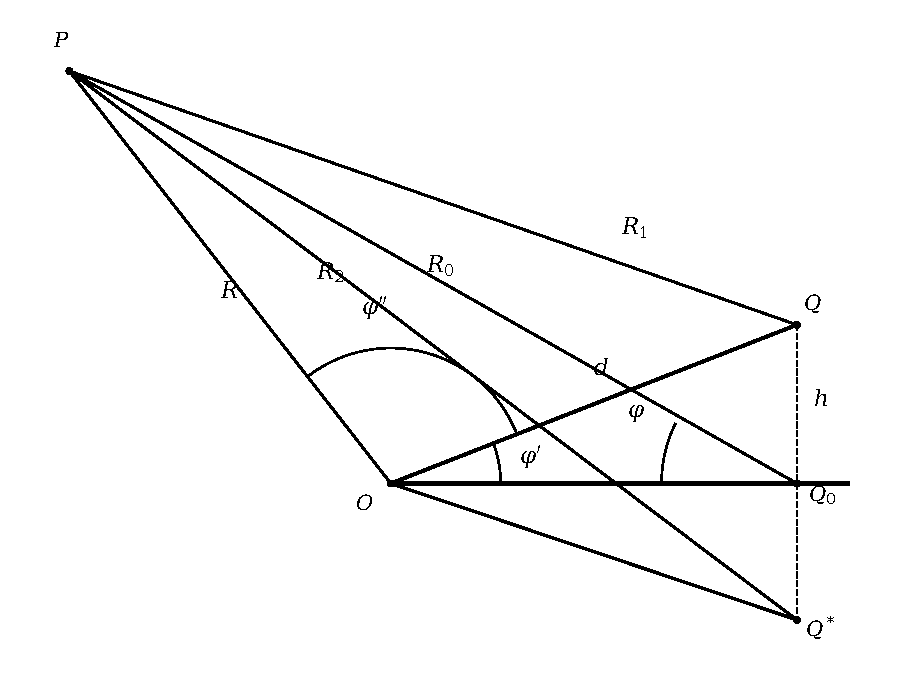
\includegraphics[width=.95\linewidth]{images/recreated/b-0135-fig46.pdf}

\raggedright Figure 46. Diffraction of a cylindrical wave by a half-plane. $Q$ is the source, $Q^*$ is the mirror image of the source, and $P$ is the observation point.
\end{minipage}\hfill\begin{minipage}[t]{.48\linewidth}\vspace{0pt}
to be a plane wave on the section from the edge of the half-plane to the point $Q$. In this case, in accordance with \S\ 1 and \S\ 2 the field created by it at the point $Q$ will equal
\end{minipage}
\[\left.\begin{aligned}E_z(Q)&=E_{0z}(0)[u(d,\varphi'-\varphi'')-u(d,\varphi'+\varphi'')],\\H_z(Q)&=H_{0z}(0)[u(d,\varphi'-\varphi'')+u(d,\varphi'+\varphi'')].\end{aligned}\right\}\tag{20.08}\]
The functions $u$ introduced here are determined (for the values $0\leq\varphi''\leq\pi$) by the equations
\[\left.\begin{aligned}
u(d,\varphi'-\varphi'')&=e^{-ikd\cos(\varphi'-\varphi'')}\frac{e^{-i\pi/4}}{\sqrt\pi}\int_{\infty\cos\frac{\varphi'-\varphi''}2}^{\sqrt{2kd}\cos\frac{\varphi'-\varphi''}2}e^{iq^2}dq\\
&\quad+\begin{cases}e^{-ikd\cos(\varphi'-\varphi'')}&\text{with }0\leq\varphi'\leq\pi+\varphi'',\\0&\text{with }\pi+\varphi''<\varphi'\leq2\pi,\end{cases}\\
u(d,\varphi'+\varphi'')&=e^{-ikd\cos(\varphi'+\varphi'')}\frac{e^{-i\pi/4}}{\sqrt\pi}\int_{\infty\cos\frac{\varphi'+\varphi''}2}^{\sqrt{2kd}\cos\frac{\varphi'+\varphi''}2}e^{iq^2}dq\\
&\quad+\begin{cases}e^{-ikd\cos(\varphi'+\varphi'')}&\text{with }0\leq\varphi'\leq\pi-\varphi'',\\0&\text{with }\pi-\varphi''<\varphi'\leq2\pi,\end{cases}
\end{aligned}\right\}\tag{20.09}\]
and the quantities $E_z(0)$ and $H_z(0)$ are the values of the primary field created by the auxiliary filament at points corresponding to the half-plane's edge. In accordance with Equations (1.21) and (1.22), this field may be represented when $kR\gg1$ in the form
\[\left.\begin{aligned}E_{0z}(0)&=ik^2p_{0z}\sqrt{\frac{2\pi}{kR}}e^{i(kR-\pi/4)},\\H_{0z}(0)&=ik^2m_{0z}\sqrt{\frac{2\pi}{kR}}e^{i(kR-\pi/4)}.\end{aligned}\right\}\tag{20.10}\]
\end{scanpage}
